\documentclass[12pt]{article}
\usepackage{amsmath,amssymb}
\usepackage{tikz}
\usetikzlibrary{arrows.meta, positioning, calc, decorations.markings}
\usepackage[margin=1in]{geometry}

\title{Notes on the Hodge-deRham Complex}

\author{John A. Janik}

\begin{document}
	
\maketitle

\begin{center}
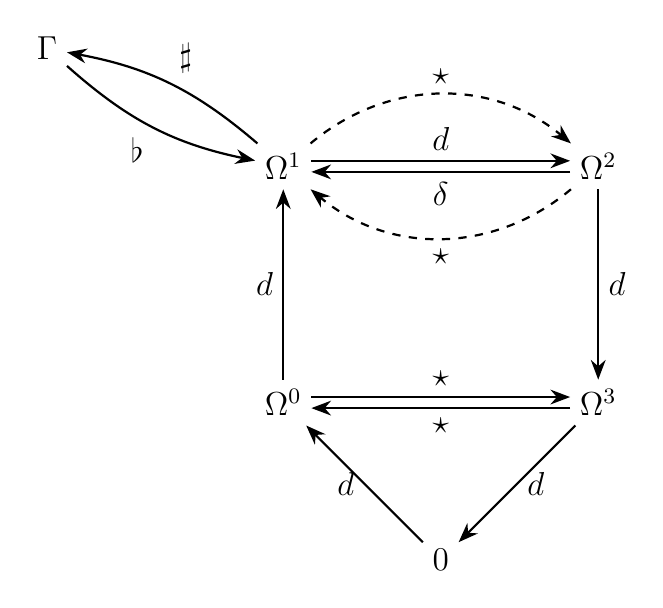
\begin{tikzpicture}[
    node distance=2.5cm and 3cm,
    every node/.style={font=\large},
    % Standard arrow
    arrow/.style={-{Stealth[length=2.5mm]}, thick},
    % Musical isomorphism arrows (decorative)
    musical/.style={-{Stealth[length=2mm, width=2mm]}, thick, 
                    looseness=0.8},
    % Double parallel arrows style
    parallel shift/.style={transform canvas={yshift=#1}}
]

% === NODES ===

% Zero at bottom center
\node (zero) at (0,-3.5) {$0$};

% Middle row: Ω⁰ and Ω³
\node (omega0) at (-2, -1.5) {$\Omega^0$};
\node (omega3) at (2, -1.5) {$\Omega^3$};

% Top row: $\omega^{1}$ and $\omega^{2}$
\node (omega1) at (-2, 1.5) {$\Omega^1$};
\node (omega2) at (2, 1.5) {$\Omega^2$};

% Gamma in upper left corner
\node (Gamma) at (-5, 3) {$\Gamma$};

% === DE RHAM COMPLEX ARROWS (d) ===

% 0 → Ω⁰
\draw[arrow] (zero) -- node[midway, left] {$d$} (omega0);

% Ω⁰ → $\omega^{1}$
\draw[arrow] (omega0) -- node[midway, left] {$d$} (omega1);

% $\omega^{1}$ → $\omega^{2}$ (upper parallel arrow)
\draw[arrow, parallel shift=2pt] (omega1) -- node[midway, above] {$d$} (omega2);

% $\omega^{2}$ → $\omega^{1}$ (lower parallel arrow, reversed for codifferential δ)
\draw[arrow, parallel shift=-2pt] (omega2) -- node[midway, below] {$\delta$} (omega1);

% $\omega^{2}$ → Ω³
\draw[arrow] (omega2) -- node[midway, right] {$d$} (omega3);

% Ω³ → 0
\draw[arrow] (omega3) -- node[midway, right] {$d$} (zero);

% === HODGE STAR ARROWS (★) ===

% Ω⁰ ↔ Ω³ (horizontal, parallel)
\draw[arrow, parallel shift=2pt] (omega0) -- node[midway, above] {$\star$} (omega3);
\draw[arrow, parallel shift=-2pt] (omega3) -- node[midway, below] {$\star$} (omega0);

% $\omega^{1}$ ↔ $\omega^{2}$ - already have d/δ, so we can add curved ★ or skip
% If you want ★ between $\omega^{1}$ and $\omega^{2}$, we need to distinguish from d/δ
% Option: use dashed or different style
\draw[arrow, dashed, bend left=40] (omega1) to node[midway, above] {$\star$} (omega2);
\draw[arrow, dashed, bend left=40] (omega2) to node[midway, below] {$\star$} (omega1);

% === MUSICAL ISOMORPHISMS (♭ and ♯) ===

% $\Gamma$ → $\omega^{1}$ (flat: ♭)
\draw[-{Stealth[length=2.5mm]}, thick, bend right=15] 
    (Gamma) to node[midway, below left] {$\flat$} (omega1);

% $\omega^{1}$ → $\Gamma$ (sharp: ♯)  
\draw[-{Stealth[length=2.5mm]}, thick, bend right=15] 
    (omega1) to node[midway, above right] {$\sharp$} (Gamma);

\end{tikzpicture}
\end{center}

\vspace{1cm}

% === CLEANER VERSION 2: More symmetric layout ===

\begin{center}
\textbf{Alternative Layout (Diamond with 0 centered at bottom)}
\end{center}

\begin{center}
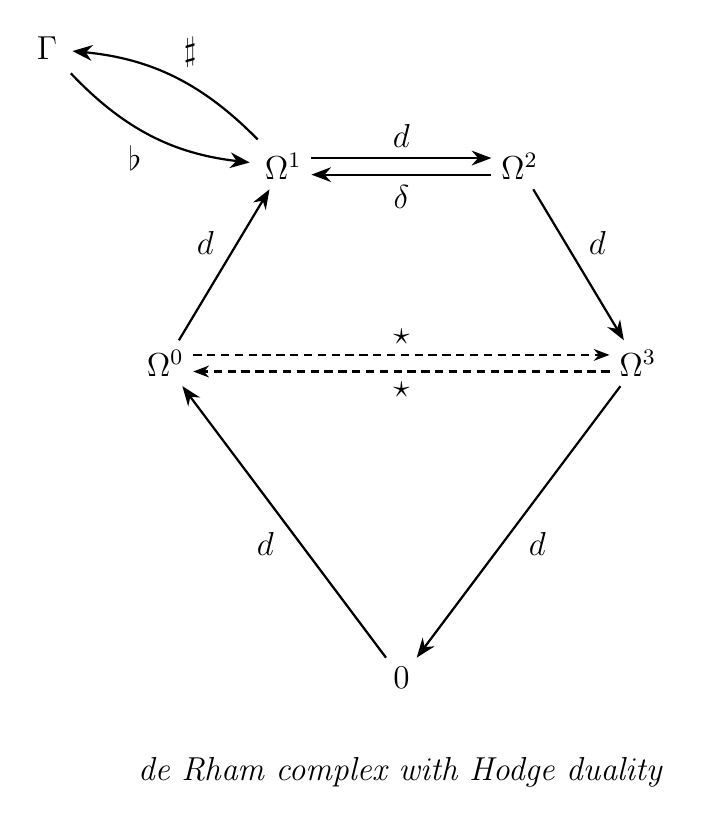
\begin{tikzpicture}[
    node distance=2cm,
    every node/.style={font=\large},
    arrow/.style={-{Stealth[length=2.5mm]}, thick},
    homark/.style={-{Stealth[length=2mm]}, thick, densely dashed},
    parallel shift/.style={transform canvas={yshift=#1}}
]

% === NODES in diamond arrangement ===

% Zero at bottom center
\node (zero) at (0,-4) {$0$};

% Ω⁰ at left
\node (omega0) at (-3, 0) {$\Omega^0$};

% Ω³ at right  
\node (omega3) at (3, 0) {$\Omega^3$};

% $\omega^{1}$ at top-left
\node (omega1) at (-1.5, 2.5) {$\Omega^1$};

% $\omega^{2}$ at top-right
\node (omega2) at (1.5, 2.5) {$\Omega^2$};

% Gamma in upper left corner
\node (Gamma) at (-4.5, 4) {$\Gamma$};

% === DE RHAM COMPLEX (d arrows) ===

% 0 → Ω⁰ 
\draw[arrow] (zero) -- node[midway, below left] {$d$} (omega0);

% Ω⁰ → $\omega^{1}$
\draw[arrow] (omega0) -- node[midway, above left] {$d$} (omega1);

% $\omega^{1}$ → $\omega^{2}$ (parallel pair)
\draw[arrow, parallel shift=3pt] (omega1) -- node[midway, above] {$d$} (omega2);
\draw[arrow, parallel shift=-3pt] (omega2) -- node[midway, below] {$\delta$} (omega1);

% $\omega^{2}$ → Ω³
\draw[arrow] (omega2) -- node[midway, above right] {$d$} (omega3);

% Ω³ → 0
\draw[arrow] (omega3) -- node[midway, below right] {$d$} (zero);

% === HODGE STAR (★) ===

% Ω⁰ ↔ Ω³ (through center, parallel)
\draw[homark, parallel shift=3pt] (omega0) -- node[midway, above] {$\star$} (omega3);
\draw[homark, parallel shift=-3pt] (omega3) -- node[midway, below] {$\star$} (omega0);

% $\omega^{1}$ ↔ $\omega^{2}$ already shown with d/δ; ★ is implicit via δ = ★d★

% === MUSICAL ISOMORPHISMS ===

% Use nice curved arrows
\draw[-{Stealth[length=2.5mm, width=2mm]}, thick, shorten >=2pt, shorten <=2pt] 
    (Gamma) to[bend right=20] node[midway, below left] {$\flat$} (omega1);
    
\draw[-{Stealth[length=2.5mm, width=2mm]}, thick, shorten >=2pt, shorten <=2pt] 
    (omega1) to[bend right=20] node[midway, above right] {$\sharp$} (Gamma);

% === LABELS ===
\node at (0, -5.2) {\textit{de Rham complex with Hodge duality}};

\end{tikzpicture}
\end{center}

\vspace{1cm}

% === VERSION 3: Most polished ===

\begin{center}
\textbf{Final Version}
\end{center}

\begin{center}
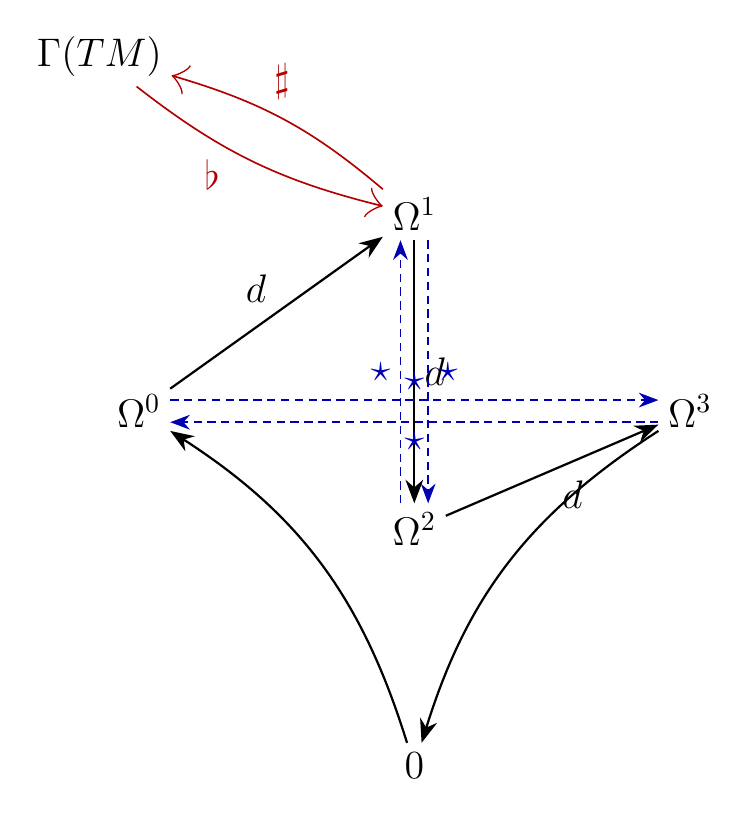
\begin{tikzpicture}[
    every node/.style={font=\Large},
    arrow/.style={-{Stealth[length=3mm]}, line width=0.8pt},
    star/.style={-{Stealth[length=2.5mm]}, line width=0.6pt, densely dashed, blue!70!black},
    musical/.style={-{Classical TikZ Rightarrow[length=2mm]}, line width=0.6pt, red!70!black},
    shift up/.style={transform canvas={yshift=4pt}},
    shift down/.style={transform canvas={yshift=-4pt}}
]

% === NODES ===

% Zero at bottom center
\node (zero) at (0,-4.5) {\Large $0$};

% Diamond arrangement
\node (omega0) at (-3.5, 0) {$\Omega^0$};
\node (omega3) at (3.5, 0) {$\Omega^3$};
\node (omega1) at (0, 2.5) {$\Omega^1$};
\node (omega2) at (0, -1.5) {$\Omega^2$};

% Gamma upper left
\node (Gamma) at (-4, 4.5) {$\Gamma(TM)$};

% === DE RHAM SEQUENCE ===

% 0 → Ω⁰
\draw[arrow] (zero) to[bend right=20] node[midway, left] {$$} (omega0);

% Ω⁰ → $\omega^{1}$  
\draw[arrow] (omega0) -- node[midway, above left] {$d$} (omega1);

% $\omega^{1}$ → $\omega^{2}$ 
\draw[arrow] (omega1) -- node[midway, right] {$d$} (omega2);

% $\omega^{2}$ → Ω³
\draw[arrow] (omega2) -- node[midway, below right] {$d$} (omega3);

% Ω³ → 0
\draw[arrow] (omega3) to[bend right=20] node[midway, right] {$$} (zero);

% === HODGE STAR === 

% Ω⁰ ↔ Ω³ (horizontal pair through middle)
\draw[star, shift up] (omega0) -- node[midway, above] {$\star$} (omega3);
\draw[star, shift down] (omega3) -- node[midway, below] {$\star$} (omega0);

% $\omega^{1}$ ↔ $\omega^{2}$ (vertical pair)
\draw[star, transform canvas={xshift=5pt}] (omega1) -- node[midway, right] {$\star$} (omega2);
\draw[star, transform canvas={xshift=-5pt}] (omega2) -- node[midway, left] {$\star$} (omega1);

% === MUSICAL ISOMORPHISMS ===

\draw[musical] (Gamma) to[bend right=12] node[pos=0.4, below left] {$\flat$} (omega1);
\draw[musical] (omega1) to[bend right=12] node[pos=0.6, above right] {$\sharp$} (Gamma);

\end{tikzpicture}
\end{center}

\section{Physical Significance of the $\omega^{2}$-Centric Diagram}

Placing $\omega^{2}$ at the geometric center of the diagram changes our perspective to reveal deep physical significance.

\subsection*{Why $\omega^{2}$ is Central}

\subsubsection*{1. \textbf{Field Strength Lives in $\omega^{2}$}}

In gauge theory, the hierarchy is:
\[
\underbrace{\Omega^0}_{\text{gauge function}} \xrightarrow{d} 
\underbrace{\Omega^1}_{\text{potential } A} \xrightarrow{d} 
\underbrace{\Omega^2}_{\text{field strength } F} \xrightarrow{d} 
\underbrace{\Omega^3}_{\text{Bianchi } dF=0}
\]

The \textbf{physics} (energy, equations of motion, observables) lives at $\omega^{2}$:
\begin{itemize}
	\item Electromagnetic field: $F = dA \in \Omega^2$
	\item Yang-Mills curvature: $F = dA + A \wedge A \in \Omega^2$
	\item Riemann curvature: $R^a{}_b \in \Omega^2(\mathfrak{so}(n))$
\end{itemize}

\subsubsection*{2. \textbf{$\omega^{2}$ is the "Self-Dual" Level (in 4D)}}

In 4 dimensions, the Hodge star satisfies:
\[
\star: \Omega^2 \to \Omega^2, \quad \star^2 = +1 \text{ (Euclidean) or } -1 \text{ (Lorentzian)}
\]

This allows decomposition into \textbf{self-dual} and \textbf{anti-self-dual} parts:
\[
\Omega^2 = \Omega^2_+ \oplus \Omega^2_-
\]

This is central to:
\begin{itemize}
	\item Instantons ($F = \star F$)
	\item Twistor theory
	\item Chiral structure of spinors
	\item Donaldson theory of 4-manifolds
\end{itemize}

\subsubsection*{3. \textbf{Symplectic Structure}}

In Hamiltonian mechanics, everything revolves around $\omega \in \Omega^2(T^*M)$:
\[
\omega = dp_i \wedge dq^i
\]

The symplectic form is a \textbf{closed, non-degenerate 2-form}. Phase space geometry is fundamentally $\omega^{2}$-geometry.

\subsubsection*{4. \textbf{The "Flux" Interpretation}}

\begin{center}
	\begin{tabular}{c|c|c}
		\hline
		\textbf{Form} & \textbf{Integrates over} & \textbf{Physical meaning} \\
		\hline
		$\Omega^0$ & point & field value \\
		$\Omega^1$ & curve & work, circulation \\
		$\boldsymbol{\Omega^2}$ & \textbf{surface} & \textbf{flux} \\
		$\Omega^3$ & volume & total charge/mass \\
		\hline
	\end{tabular}
\end{center}

Flux through surfaces is the natural "middle" concept—it connects local (differential) to global (integral) physics via Stokes' theorem.

\subsubsection*{5. \textbf{In 3D: The Pseudovector Level}}

In 3 dimensions:
\[
\star: \Omega^1 \leftrightarrow \Omega^2
\]

\begin{center}
	\begin{tabular}{c|c}
		\hline
		$\omega^{1}$ (polar vectors) & $\omega^{2}$ (axial vectors) \\
		\hline
		Electric field $\mathbf{E}$ & Magnetic field $\mathbf{B}$ \\
		Velocity $\mathbf{v}$ & Vorticity $\boldsymbol{\omega}$ \\
		Force $\mathbf{F}$ & Torque $\boldsymbol{\tau}$ \\
		Momentum $\mathbf{p}$ & Angular momentum $\mathbf{L}$ \\
		\hline
	\end{tabular}
\end{center}

The $\omega^{1}$ $\leftrightarrow$ $\omega^{2}$ duality is the \textbf{polar/axial} or \textbf{vector/pseudovector} distinction.

\hrulefill

\subsection*{The Diagram's Physical Meaning}

\begin{center}
	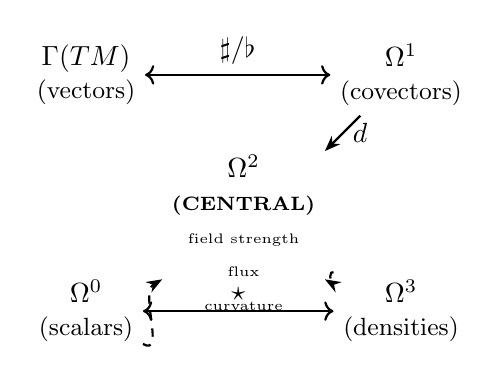
\begin{tikzpicture}[
		node distance=1.2cm,
		every node/.style={font=\normalsize, align=center},
		arrow/.style={-{Stealth[length=2mm]}, thick},
		small node/.style={font=\small}
		]
		
		% Nodes
		\node (GammaTM) at (-2, 3) {$\Gamma(TM)$ \\ \small (vectors)};
		\node (omega1) at (2, 3) {$\Omega^1$ \\ \small (covectors)};
		\node (omega0) at (-2, 0) {$\Omega^0$ \\ \small (scalars)};
		\node (omega3) at (2, 0) {$\Omega^3$ \\ \small (densities)};
		\node (omega2) at (0, 1) {$\Omega^2$ \\ \scriptsize \textbf{(CENTRAL)} \\ \tiny field strength \\ \tiny flux \\ \tiny curvature};
		
		% Musical isomorphisms
		\draw[arrow, <->] (GammaTM) -- node[midway, above] {$\sharp/\flat$} (omega1);
		
		% Exterior derivative
		\draw[arrow] (omega1) -- node[midway, right] {$d$} (omega2);
		
		% Hodge star
		\draw[arrow, <->] (omega0) -- node[midway, above] {$\star$} (omega3);
		\draw[arrow, dashed] (omega0) to[out=-30, in=210] (omega2);
		\draw[arrow, dashed] (omega3) to[out=150, in=-30] (omega2);
		
	\end{tikzpicture}
\end{center}

\textbf{Interpretation:}
\begin{itemize}
	\item $\mathbf{\Omega^0}$ (left): Potentials, scalar fields, gauge functions
	\item $\mathbf{\Omega^3}$ (right): Densities, sources, charges (integrated quantities)
	\item $\mathbf{\Omega^1}$ (top): The "configuration" level—connections, velocities
	\item $\mathbf{\Omega^2}$ (center): The "dynamics" level—field strengths, curvatures, fluxes
	\item $\mathbf{\Gamma(TM)}$ (upper left): Vectors, related to $\omega^{1}$ by the metric via musical isomorphisms
\end{itemize}

The \textbf{musical isomorphisms} ($\flat$ and $\sharp$) require a metric to convert between vectors and covectors. The \textbf{Hodge star} also requires a metric and orientation.



\end{document}
